\documentclass[reqno,final,11pt]{amsart}
%% Packages
\usepackage{natbib}  %Nature-like bibliography
\usepackage{fancyhdr} %Headers
\usepackage{color} %Color definition
\usepackage{hyperref} %Internal and external links
\usepackage{graphicx} %Graphics inclusion
\usepackage{geometry}
\geometry{
  top=1in,            
  inner=1in,
  outer=1in,
  bottom=1in,
  headheight=3ex,       
  headsep=2ex,          
}
\usepackage[utf8]{inputenc}
\usepackage[T1]{fontenc}

%%%%%%%%%%%%%%%%%%%%%%%%%%%%%%%%%%%%%
%% Author packages
%%%%%%%%%%%%%%%%%%%%%%%%%%%%%%%%%%%%%
% Please remove packages that are not useD
\usepackage{tikz}
\usetikzlibrary{calc,shapes,backgrounds,arrows}
\usepackage{amssymb}

%%%%%%%%%%%%%%%%%%%%%%%%%%%%%%%%%%%%%


%% Definition of colors for links
\definecolor{aleacolor}{rgb}{0.16,0.59,0.78}

%% Settings for hyperref package
\hypersetup{
breaklinks,
colorlinks=true,
linkcolor=aleacolor,
urlcolor=aleacolor,
citecolor=aleacolor}

%% Settings for fancyhdr package
%\renewcommand{\headheight}{11pt}
\pagestyle{fancy} \fancyhf{} \fancyhead[RO,LE]{\small\thepage}
\fancyhead[RE]{\small\shortauthors} \fancyhead[LO]{\small\shorttitle}

%% Settings for natbib package
\renewcommand{\cite}{\citet}

%% Setting the theorem-like environments
\theoremstyle{plain}
\newtheorem{theorem}{Theorem}[section]                                          
\newtheorem{proposition}[theorem]{Proposition}                          
\newtheorem{lemma}[theorem]{Lemma}
\newtheorem{corollary}[theorem]{Corollary}
\newtheorem{conjecture}[theorem]{Conjecture}
\theoremstyle{definition}
\newtheorem{definition}[theorem]{Definition}
\theoremstyle{remark}
\newtheorem{remark}[theorem]{Remark}
\newtheorem{example}[theorem]{Example}

%% Numbering
\makeatletter \@addtoreset{equation}{section} \makeatother
\renewcommand\theequation{\thesection.\arabic{equation}}
\renewcommand\thefigure{\thesection.\arabic{figure}}
\renewcommand\thetable{\thesection.\arabic{table}}

%% First page header, modify the link w.r.t. volume number
\newcommand{\aleaIndex}[1]{\href{http://alea.impa.br/english/index_v23.htm}{\bf 23}}
\newcommand{\aleaDOI}[1]{\href{https://doi.org/10.30757/ALEA.v23-}{DOI: 10.30757/ALEA.v23-}}
\eheader{ALEA, Lat. Am. J. Probab. Math. Stat.}{\aleaIndex{23}}{2026}{1}{4}{\aleaDOI}
%% Uncomment the following line to include Alea logo
\elogo{\parbox[c]{180pt}{
\includegraphics[width=170pt]{logo.pdf}}} % 3 centimeters = 85.0393701 PostScript points

%%%%%%%%%%%%%%%%%%%%%%%%%%%%%%%%%%%%%
%% Author commands and definitions
%%%%%%%%%%%%%%%%%%%%%%%%%%%%%%%%%%%%%
% add your custom commands; please avoid:
% - creating commands that are not used
% - using \renewcommand, since it can create conflicts
\newcommand{\tildeurl}{\raisebox{0.5ex}\texttildelow} % tilde for url addresses
\newcommand{\N}{\mathbb{Z}_{+}}
\newcommand{\Z}{\mathbb{Z}}
\newcommand{\Zd}{\mathbb{Z}^d}
\newcommand{\R}{\mathbb{R}}

%%%%%%%%%%%%%%%%%%%%%%%%%%%%%%%%%%%%%
\date{DATE; accepted DATE; published under license
\href{https://creativecommons.org/licenses/by/4.0/}{\textup{CC BY 4.0}}} %%% to be modified by the editor

\begin{document}

\title[Short Title]{Complete Title of this Article}

\author{First Author}
\address{First Author Adress}
\email{first@email.com} 
\urladdr{\href{http://First.com/~address}{http://first.com/{\tildeurl}address}} 

\author{Second Author}
\address{Second Author Adress}
\email{second@email.com} 
\urladdr{\href{http://second.com/~address}{http://second.com/{\tildeurl}address}} 



\author{Third Author}
\address{Third Author Adress}
\email{third@email.com} 
\urladdr{\href{http://third.com/~address}{http://third.com/{\tildeurl}address}} 


\thanks{First Author has been supported by some agency. Second Author and Third Author have been supported by some other grant}
\subjclass[2020]{82C44, 60K35, 60G70} 
\keywords{Random dynamics, random environments, scaling limit}





\begin{abstract}
  This is an example of ALEA's \LaTeX style available at ALEA's
  website. Compile it preferentially using {\tt pdflatex}.

    
   
\end{abstract}

\maketitle

\section{Introduction}


\subsection{Citations}
\label{ss_citations}

\begin{itemize}
\item Compile bibliography using {\tt bibtex} (to find bibliographical entries,
\href{https://mathscinet.ams.org/mathscinet/}{MathSciNet} database may be
        useful).

\item Whenever it is possible, provide a DOI reference for the citation.

\item In this latex style the {\tt $\backslash$cite} command creates
citations using the name of the author and the date of publishing, for
example \cite{MR1557756}.

\item We can also group citations as \cite{MR1557756,MR1557978,MR1557852}.

\item If the citation is between parentheses, use the command
{\tt $\backslash$citealp} to avoid the double parentheses (for example
\citealp{MR0050410}).

\item Please notice that if your original manuscript had numbered
citations, changing it to ALEAs style \textbf{may cause conflicts}: e.g.,
`reference Scott [1]' will become `reference Scott \cite{MR1557756}'. 

\item It is very important to attach the file \emph{.bib} with all references
(see {\tt example.bib}).
\end{itemize}

\subsection{Graphics}
\label{ss_graphics}
\begin{itemize}
\item To create graphics, include images preferentially in \texttt{Tikz}
(see Figure~\ref{fig1}) or png (see Figure~\ref{fig2}), but other formats
may be also accepted.

\item Please include all files of external figures in your final submission.
\end{itemize}

\begin{figure}[!htb]
\centering
\begin{tikzpicture}
\draw[->] (-2,0) -- (6,0) node[anchor=north] {$x$};
\draw	(0,0) node[anchor=north] {0}
		(2,0) node[anchor=north] {$\frac{1}{2}$}
		(4,0) node[anchor=north] {1}
		(0,3) node[anchor= east] {\scriptsize $\log 2$};
\draw[->] (0,0) -- (0,4) node[anchor=east] {$I$};
\draw[dotted] (4,0) -- (4,4);
\draw[-, thick] (4,5) -- (6,5) ;
\filldraw[fill=white, draw=black] (4,5) circle (2pt);
\draw (6.5,5) node {$+\infty$}; %label
\draw[-,thick] (-2,5) -- (0,5) ;
\filldraw[fill=white, draw=black] (0,5) circle (2pt);
\draw (-2.5,5) node {$+\infty$}; %label
\draw[-,thick]  (0,3) parabola[bend at end] (2,0);
\filldraw[fill=black, draw=black] (0,3) circle (2pt);
\draw[thick,-]  (2,0) parabola (4,3);
\filldraw[fill=black, draw=black] (4,3) circle (2pt);
\end{tikzpicture}
\caption{Rate function $I:\mathbb R\to [0,\infty]$}
\label{fig1}
\end{figure}



\subsection{Statements}
\label{ss_statements}

\begin{itemize}
\item Tagged and untagged formulas are presented in the next section, where
we further illustrate the use of the commands {\tt $\backslash$section},
{\tt $\backslash$subsection}, and  environments as
{\tt $\backslash$begin$\{$theorem$\}$} {\tt ...}
{\tt $\backslash$end$\{$theorem$\}$}.

\item Theorems, lemmas, propositions etc.\ should be referred as
Theorem~\ref{thm1} for instance, and sections as Section~\ref{sec2}
for example.

\item Make reference to equations using \texttt{$\backslash$eqref$\{\}$} and
make references to theorem, lemmas, etc., using \texttt{$\backslash$ref$\{\}$}.
    
\item \textbf{Avoid using} \texttt{$\backslash$left...$\backslash$right}.
Prefer using predetermined sizes, such as \texttt{$\backslash$big$($},
\texttt{$\backslash$Big$($}, \texttt{$\backslash$bigg$($} and
\texttt{$\backslash$Bigg$($}.

\item \textbf{Do not use} the environment \texttt{$\backslash$begin$\{$eqnarray$\}$}
\texttt{...} \texttt{$\backslash$end$\{$eqnarray$\}$} and prefer instead the
environments \texttt{$\backslash$begin$\{$align$\}$}\texttt{...$\backslash$end$\{$align$\}$}
or \texttt{$\backslash$begin$\{$align*$\}$...$\backslash$end$\{$align*$\}$}
or \texttt{$\backslash$begin$\{$multline$\}$} \texttt{...} \texttt{$\backslash$end$\{$multline$\}$}
or \texttt{$\backslash$begin$\{$multline*$\}$...$\backslash$end$\{$multline*$\}$}.
\end{itemize}
  



\section{Dummy text example}\label{sec2}

Lorem ipsum dolor sit amet, consectetur adipiscing elit. Integer sit amet justo id sapien fringilla hendrerit eu quis arcu. Duis tristique mollis tortor, ac aliquet justo faucibus et. Pellentesque elementum vulputate malesuada. Phasellus bibendum commodo sem, vitae tincidunt nulla vehicula vehicula. Integer mattis sapien risus, a molestie leo. Sed tortor ante, sagittis ac imperdiet non, ultrices ut dolor. Nunc ut velit vel massa euismod hendrerit. Nulla iaculis tellus magna. Fusce vitae enim sapien. Mauris ac dignissim leo.


 Nullam et nisi sit amet lectus lacinia porta. Donec non quam at risus convallis fringilla id sit amet metus. Donec ut magna magna. Praesent velit quam, molestie vitae venenatis sed, scelerisque eu nisi. Sed eleifend orci at dui lobortis mollis viverra augue luctus. Vivamus convallis nulla id diam molestie gravida. Mauris lorem sem, tincidunt dictum vulputate eu, feugiat vitae mi. Donec leo lacus, tristique sit amet ullamcorper et, egestas vitae leo. Pellentesque ultricies sollicitudin augue ac posuere. Donec condimentum, sem id semper vehicula, dui sapien dapibus augue, non facilisis tellus libero non felis. Integer vitae velit in tortor aliquam tempus nec nec ante.

The infinitesimal generator $\big(A_Lf\big)(n)$ is equal to
\begin{align}
 & \frac{A}{L^a}\Big[f(n_{\delta(-)}+n_{-L},0,n_{-L+1},\ldots,n_{\delta(+)})-f(n)\Big]\label{eq01}\\
& +\frac{B}{L^b}\Big[f(n_{\delta(-)},\ldots,n_{L-1},0,n_{\delta(+)}+n_L)-f(n)\Big] \notag \\
&
 +\sum_{j=-L}^L\frac{1}{n_j+n_{j+1}+1}\sum_{q=0}^{n_j+n_{j+1}}\!\!\Big[
f(n_{\delta(-)},n_{-L},\ldots,n_{i-1},q,n_i+n_{i+1}-q,\ldots,n_{\delta(+)})-f(n)\Big]\,,\label{eq02}
\end{align}
cras et lacus elit, et accumsan velit. Morbi sed nunc sit amet ipsum dapibus blandit et id est. Suspendisse nec justo sapien, vel ullamcorper risus. In hac habitasse platea dictumst. Duis gravida tempor aliquam. Sed in nisi sit amet lectus ultricies luctus eu quis nisl. Morbi nec sollicitudin metus. Aliquam pellentesque, ligula id auctor tincidunt, magna nisi adipiscing ligula, at egestas sapien metus ut felis. Phasellus porttitor commodo massa, pharetra congue diam dapibus pellentesque. In vitae mauris odio, euismod luctus turpis. Nam at mi nunc, vitae fringilla tellus. Vivamus tincidunt gravida imperdiet. Donec mauris arcu, rutrum sed semper sit amet, tempus sit amet nibh. Nulla vehicula pharetra lorem a pharetra. Etiam et metus mauris, nec ultrices ipsum. Nullam interdum pulvinar consequat. Phasellus varius turpis eros. Duis quis erat eu eros tristique ultricies. Mauris dignissim egestas fermentum. Donec quis nisi non velit vestibulum lacinia (c.f.\ Figure~\ref{fig2}).
\begin{figure}[!htb]
\centering
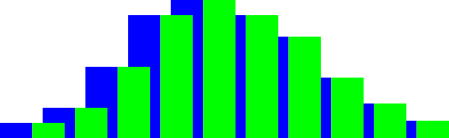
\includegraphics[scale=0.75]{image.png} 
\caption{Some distribution}
\label{fig2}
\end{figure}



\subsection{Alea jacta est}
Fusce id eros vel lorem iaculis vulputate. Mauris imperdiet massa nulla, et dapibus tortor. Cum sociis natoque penatibus et magnis dis parturient montes, nascetur ridiculus mus. Mauris dictum consequat dui, ut consequat ligula convallis ut. Phasellus nisl magna, venenatis eget pharetra ac, commodo eu odio. Mauris porta pharetra metus. Nulla molestie porta erat, in tincidunt sem consequat ut. Morbi mollis facilisis imperdiet. Nunc vulputate, urna at rhoncus ullamcorper, lectus lectus facilisis massa, id condimentum est ipsum sed dolor. Sed accumsan ligula quis urna ornare ut euismod nisi venenatis. Morbi nulla nibh, tincidunt sit amet dignissim a, rhoncus a nibh.
\begin{lemma}\label{lemma1}
 Pellentesque nibh turpis, $\Omega \neq \varnothing$, Vivamus vitae massa a lorem eleifend dignissim eget eu orci.  Nunc vel:
\begin{align*}
\mathbb P(X_{n+1} = x \,|\, \mathcal G_n)\; =\; \frac{e^{\beta \,c_n(X_n, x)}}{
	\sum_{y\sim X_n} e^{\beta \,c_n(X_n, y)}}\,.
\end{align*}
\end{lemma}
\begin{proof}
Sed a elit quis enim tincidunt dignissim vitae eget erat. Quisque tempus ante semper dolor scelerisque mollis. Nulla libero odio, vulputate non iaculis a, placerat at justo. Praesent luctus eleifend purus vel elementum. Nulla enim ligula, sagittis ut pretium a, scelerisque ut eros. 
\begin{align}
|F|\;\lesssim\; &  \Big(\mathbb P_0\big[X_{s_2n^2}=-1\big]+\mathbb P_0\big[X_{s_2n^2}=0\big]\Big) \notag\\
&\times \bigg(\dfrac{1}{((s_1-s_2)n^2)^2}+\Big|K_{(s_1-s_2)n^2}(0)-K_{(s_1-s_2)n^2}(1)\Big|\bigg) \notag \\
\;\lesssim\;&\dfrac{1}{\sqrt{ s_2}}\cdot \dfrac{1}{(s_1-s_2)^{3/2}n^4}\,.\label{eq03}
\end{align}
Sed auctor justo id elit volutpat bibendum. In aliquet dui vel mi consectetur dictum. Vestibulum vel lectus ut lacus porttitor bibendum sit amet nec erat \eqref{eq03}. Fusce nec elit ante, sit amet ullamcorper nisl. Sed a tellus sed augue molestie accumsan.
\begin{align*}
\sum_{k=0}^n\binom{n}{k}a^k{(1-a)}^{n-k}\;=\; 1\,.
\end{align*}

Praesent nisi erat, sollicitudin eu lacinia quis, tempus eu velit. 
Nulla magna erat, rhoncus eu suscipit et, 
rutrum vitae turpis. Vivamus sed neque leo. Donec id felis ut est viverra.
\end{proof}
\begin{theorem}\label{thm1}
 Lorem ipsum dolor sit amet $\gamma \in \R$, consectetur adipiscing elit $j\in\N$, $\tau\in\Z$. Pellentesque nibh turpis, sagittis ac scelerisque et, rhoncus et enim. Nunc vel:
\begin{align}\label{eq04}
\lim_{n\to\infty} \frac{1}{a_n}\log \Big(\int_X e^{a_nF(x)}\,P_n(dx)\Big)\;=\;\sup_{x\in X}\Big\{ F(x)-I(x)\Big\}.
\end{align}
\end{theorem}
\begin{proof}
By Lemma~\ref{lemma1},  aenean consequat, urna in congue viverra, enim nunc suscipit lorem \eqref{eq04}.
\end{proof}

\section*{Acknowledgements}
The author would like to thank an anonymous referee for
pointing out several mistakes in a preliminary version.

\bibliographystyle{alea3}
\bibliography{example}


\end{document}



